\chapter{Quality Factor Measurements}\label{ch:qfactor}
As we have mentioned before resonant permittivity measurements use the resonances in an RF resonator to determine the complex permittivity of a specimen. Typically an RF resonator has multiple resonances, also called modes, which are also the degrees of freedom of the system. To model the resonances in an RF resonator we can use a simple RLC circuit, which has only one degree of freedom to describe more complicated systems.

\begin{figure}
\centering
\begin{circuitikz}
\ctikzset {bipoles/length=0.9cm}
%\draw[step=1.0,black,thin] (0,0) grid (15,10);
% Source block
\draw (2,2) to[R=$Z_0$,*-] (0,2)
			to[sV_=$U_s$] (0,0)
			to[short,-*] (2,0);
% Transmission line
\draw[<->, thick] (2,2.5) -- (4,2.5) node[midway,above] {$l$};
\draw [ultra thick] (2,2) -- (4,2);
\draw [ultra thick] (2,0) -- (4,0);
\draw (3,1) node{$Z_0, \beta$};
% Coupling network
\draw (4,2) to[L=$jX_s$,*-] (5.5,2)
		to[R=$R_s$] (7,2)
		to[short] (10,2);
\draw (4,0) to[short,*-] (10,0);
% RLC
\draw (8,2) to[R,*-*] (8,0);
\draw (9,2) to[C,*-*] (9,0);
\draw (10,2) to[L] (10,0);
\draw (9,-0.5) node{$Y(j\omega )$};
% Reference planes
\draw [thin,dashed](2,-0.5) node[below] {1} -- (2,2.5);
\draw [thin,dashed](4,-0.5) node[below] {2} -- (4,2.5);
\draw [thin,dashed](7,-0.5) node[below] {3} -- (7,2.5);

\end{circuitikz}
\caption{A simple RLC circuit, adapted from \cite{kajfez}.}\label{fig:RLC_reflect}
\end{figure}

Fig. \ref{fig:RLC_reflect} shows an example of such a simple RLC circuit \cite{kajfez}. An AC source with source impedance $Z_0$ feeds an RLC circuit using a transmission line of length $l$ and impedance $Z_0$. Depending on the coupling mechanism a lossy inductor may be used to model the coupling. 

\begin{equation}\label{eq:RLC}
f_0=\frac{1}{2\pi\sqrt{LC}}\qquad
Q_0=\frac{2\pi f_0C}{G_0}
\end{equation}

By coupling we understand the flow of power in and out of the resonator when it is excited by a source. A simple RLC circuit is capable of resonating on its own, but to measure the properties of the resonance we need to excite the resonator and measure its response. This measurement 'loads' the resonator, i.e. the power lost in the measurement increases the loss of the resonator. Therefore, we characterise a resonator through its resonant frequency $f_0$ and its unloaded quality factor $Q_0$, in case of the RLC circuit this is shown in Equation \eqref{eq:RLC}. The quality factor is a measure for the loss in a resonator and determines how fast the energy oscillating in the resonator will be lost. As can be seen in Equation \eqref{eq:Q} the quality factor $Q$ is proportional to the average energy $\overline{W}$ divided by the losses $P$ in a resonator. This ratio is also a time constant for the energy $W(t)$ oscillating in the resonator at an angular frequency $\omega_0 = 2\pi f_0$.

\begin{equation}\label{eq:Q}
Q=\frac{\omega_0\overline{W}}{P}\qquad W(t)=\overline{W} e^{-t/\tau}\qquad \tau=\frac{Q}{\omega_0}
\end{equation}

\begin{figure}
\centering
\begin{circuitikz}[american]
\ctikzset {bipoles/length=0.9cm}
%\draw[step=1.0,green,thin] (0,0) grid (10,3);
% Source block
\draw (6,0) to[short] (0,0)
		to[american current source=$i_s$] (0,2)
		to[short] (6,2);
% Equivalent shunt impedances
\draw (1,2) to[R=$G_{ex}$,*-*] (1,0);
\draw (2,2) to[L=$jB_{ex}$,*-*] (2,0);
% RLC circuit
\draw (4,2) to[R,*-*] (4,0);
\draw (5,2) to[C,*-*] (5,0);
\draw (6,2) to[L] (6,0);
\draw (5,-0.5) node{$Y(j\omega )$};
\end{circuitikz}
\caption{Thévenin equivalent circuit of Fig. \ref{fig:RLC_reflect}, shunt impedances shown in Eq. \eqref{eq:thevenin}.}\label{fig:RLC_thevenin}
\end{figure}

In case of the RLC circuit in Fig. \ref{fig:RLC_reflect} the lossy inductive coupling loads the resonator, the loaded resonator has a resonant frequency $f_L$ and a loaded quality factor $Q_L$ that is different from the unloaded resonator. Using the Thévenin equivalent circuit of Fig. \ref{fig:RLC_thevenin} it can be shown that the loading of the resonator depends on the Thévenin shunt impedances.
\begin{gather}
\shortintertext{Using a convienient expression for the admittance of the RLC circuit,}\
Y(\omega)=G+j\omega C+\frac{1}{j\omega L}=G+j\sqrt{\frac{C}{L}}(\frac{f}{f_0}-\frac{f_0}{f})=G(1+jQ_0\delta)
\shortintertext{introducing a detuning factor,}\
\delta(f)=\frac{f}{f_0}-\frac{f_0}{f}\qquad \delta(f)=0 \Leftrightarrow f=f_0
\shortintertext{we yield an expressions for $f_L$ and $Q_L$ of the loaded resonator.}\
B_{ex}+G_0Q_0\delta_L =0 \Rightarrow \delta_L(f_L)=\frac{-B_{ex}}{G_0Q_0} \qquad
Q_L=\frac{\omega C}{G}=\frac{\omega_LC}{G_0+G_{ex}}
\end{gather}\label{eq:Q_L}
We used the resonance condition $\Im(Z)=0$ for linear lumped circuits, i.e. voltage and current in the resonator are in phase. From a physical point of view this means that the electrical energy is equal to the magnetic energy in the circuit. This condition also is also satisfied by the electro-magnetic field in a cavity at resonance.
\begin{equation}\label{eq:thevenin}
i_s=\frac{U_s}{R_s+Z_0+jX_s}\qquad G_{ex}=\frac{R_s+Z_0}{(R_s+Z_0)^2+X_s^2} \qquad B_{ex}=\frac{X_s}{(R_s+Z_0)^2+X_s^2}
\end{equation}

\begin{gather}
\shortintertext{Due to the fact that the coupling only detunes a resonator lightly, we can use the first-order Taylor series}
f(\delta)\approx f_0(1+\delta/2) \Rightarrow f_L\approx f_0(1+\delta_L/2)=f_0(1-\frac{B_{ex}}{2G_0Q_0}) 
\shortintertext{to describe the detuning of the resonator. If the coupling is sufficiently small or mostly resistive, we can derive a simplified expression for $Q_L$ and introduce a coupling coefficient $\kappa$ to model the coupling of such a resonator.}
Q_L=\frac{\omega_LC}{G_0+G_{ex}}\approx\frac{\omega_0C}{G_0+G_{ex}}=Q_0\frac{1}{1+\frac{G_{ex}}{G_0}}=Q_0\frac{1}{1+\kappa}
\end{gather}

With this simple example of an RF resonator we have now introduced the concepts of resonant frequencies and quality factors of loaded and unloaded resonators. Although real RF resonators have multiple resonances, the concepts introduced here can be used to characterise each mode of a real resonator. For complex permittivity measurements we are interested in the properties of the unloaded resonator, since the coupling is usually only a mean to couple energy in and out of the resonator. In many cases the real part of the permittivity is derived from the unloaded resonant frequency and the imaginary part is derived from the unloaded quality factor \cite{kajfez, NPL}.

For the complex permittivity measurements it is vital to accurately measure these resonances. This is achieved by accurate measurements of the reflection coefficient or the transmission coefficient at ports of the resonator with vector network analysers (VNA) or similar devices. A resonator may have one or multiple ports through which measurements can be performed. Irrespective of the number of ports, measurements using the reflection coefficient are reflection-type measurements and measurements using the transmission coefficient are transmission-type measurements. 

\section{Reflection-Type Measurements}
An example for a reflection-type measurement is shown in Fig. \ref{fig:RLC_reflect}. The ideal voltage source $U_s$ with its internal resistance $Z_0$ is a representation of a reflection coefficient measurement, where the reflection coefficient is measured at reference plane (1). In Fig. \ref{fig:Smith-reflect} the Smith chart of this reflection-type measurement is illustrated. Beginning at reference plane (3) a shunt RLC circuit resembles a circle in the Smith chart when plotted over frequency, where the resonant frequency is the location on the Smith chart with the smallest reflection coefficient, marked with a cross in the Smith chart. If we assume that the series resistance $R_s$ is small, the reflection coefficient is transformed mainly by the inductive coupling of the resonator. In reference plane (2) the reflection coefficient is rotated in a clockwise direction and its diameter is changed. As we have discussed previously, this changes the resonant frequency and the quality factor of the resonator.  The resonant frequency at reference plane (2) is marked by a triangle and lies right next to the original resonant frequency of the RLC circuit, which is still marked by a cross. The resonant frequency at reference plane (2) lies also at the point with the smallest reflection coefficient. For the quality factor we can see that the coupling increases the loaded quality factor a little bit over the situation at reference plane (3), where the reference impedance led to a critically coupled resonator. Finally, the transmission line rotates the resonance circle while we move from reference plane 2 to reference plane 1. This rotation has no influence on the measurement of a resonance circle if the bandwidth of the resonance is narrow, i.e. the quality factor is high, and can be compensated by an appropriate counter-rotation \cite{kajfez}.

\begin{figure}
\centering
\begin{tikzpicture}
\def\G0{1.3}
\def\Q0{100}
\def\Ls{0.2e-9}
\def\dL{0.0018}

\pgfplotsset{every mark/.append style={solid}}
\begin{smithchart}[mark options={solid}]

%% RLC circle
\addplot[red,samples=500,domain=-0.5:0.5]({\G0 /(\G0 ^2+(\G0 *\Q0 *x)^2)}, {-\G0 *\Q0 *x/(\G0 ^2+(\G0 *\Q0 *x)^2)});
\node[red] at (0.25,0) {(3)};
% Center
\addplot[mark=x] coordinates {({\G0 /(\G0 ^2+(\G0 *\Q0 *0)^2)}, {-\G0 *\Q0 *0/(\G0 ^2+(\G0 *\Q0 *0)^2)})};
% 3dB - Points
\addplot[mark=o, dashed] coordinates {({\G0 /(\G0 ^2+(\G0 *\Q0 /\Q0 )^2)}, {-\G0 *\Q0 /\Q0 /(\G0 ^2+(\G0 *\Q0 /\Q0 )^2)}) (1,0)};
\addplot[mark=o, dashed] coordinates {({\G0 /(\G0 ^2+(\G0 *\Q0 /-\Q0 )^2)}, {\G0 *\Q0 /\Q0 /(\G0 ^2+(\G0 *\Q0 /-\Q0 )^2)}) (1,0)};
%%%%%%%%%%%%%%%%%%%%%%%%%%%%%%%%%%%%%%%%%%%%%%%%%%%%%%%%%%%%%%%%%%%%%%%%%%%%%%%%%%%%%%%%%%%%%%%%%%%%%%%%%%%%%%%%%%

%% RLC+X_s circle
\addplot[blue,samples=500,domain=-0.5:0.5]({\G0 /(\G0 ^2+(\G0 *\Q0 *x)^2)}, {-\G0 *\Q0 *x/(\G0 ^2+(\G0 *\Q0 *x)^2)+2*3.14*10e9/2*(x+sqrt(x^2+4))*\Ls /50});
\node[blue] at (0.28,0.22) {(2)};
% Center
\addplot[mark=x] coordinates {({\G0 /(\G0 ^2+(\G0 *\Q0 *0)^2)},{-\G0 *\Q0 *0/(\G0 ^2+(\G0 *\Q0 *0)^2)+2*3.14*10e9/2*(0+sqrt(0^2+4))*\Ls /50})};
% Resonant frequency (loaded)
\addplot[mark=triangle] coordinates {({\G0 /(\G0 ^2+(\G0 *\Q0 *\dL )^2)},{-\G0 *\Q0 *\dL /(\G0 ^2+(\G0 *\Q0 *\dL )^2)+2*3.14*10e9/2*(\dL +sqrt(\dL ^2+4))*\Ls /50})};
\addplot[no markers] coordinates {(0,0.2364) (1,0)};
%\addplot[no markers] coordinates {({\G0 /(\G0 ^2+(\G0 *\Q0 *0)^2)},{-\G0 *\Q0 *0/(\G0 ^2+(\G0 *\Q0 *0)^2)+2*3.14*10e9/2*(0+sqrt(0^2+4))*\Ls /50}) (1,0)};
% 3dB - Points
\addplot[mark=o, dashed] coordinates {({\G0 /(\G0 ^2+(\G0 *\Q0 /\Q0 )^2)}, {-\G0 *\Q0 /\Q0 /(\G0 ^2+(\G0 *\Q0 /\Q0 )^2)+2*3.14*10e9/2*(1/\Q0 +sqrt((1/\Q0 )^2+4))*\Ls /50}) (1,0)};
\addplot[mark=o, dashed] coordinates {({\G0 /(\G0 ^2+(\G0 *\Q0 /-\Q0 )^2)}, {\G0 *\Q0 /\Q0 /(\G0 ^2+(\G0 *\Q0 /-\Q0 )^2)+2*3.14*10e9/2*(-(1/\Q0 )+sqrt((1/\Q0 )^2+4))*\Ls /50}) (1,0)};
%%%%%%%%%%%%%%%%%%%%%%%%%%%%%%%%%%%%%%%%%%%%%%%%%%%%%%%%%%%%%%%%%%%%%%%%%%%%%%%%%%%%%%%%%%%%%%%%%%%%%%%%%%%%%%%%%%
\end{smithchart}
\end{tikzpicture}
\caption{Smith chart of a reflection-type measurement.}\label{fig:Smith-reflect}
\end{figure}

While it is possible to find the point of resonance on a Smith chart, the Smith chart does not show the frequency of the resonator at resonance. It is more convenient to take the frequency sweep over the complex reflection coefficient like in Fig. \ref{fig:resonance} and use appropriate techniques like the 3dB method to find the resonant frequency and quality factor of the resonator. We will elaborate on these techniques in this chapter. The magnitude of the reflection coefficient plot has a characteristic bell shape that reaches a minimum at the resonant frequency (again marked by an x in the plot) and the width of the bell is a measure for the quality factor of the resonator. This is the characteristic behaviour that can be observed for every resonator around its resonant frequency. We can show that a shunt RLC circuit has a similarly shaped reflection coefficient for any network that has a sufficiently flat frequency response around the resonant frequency of the RLC circuit.
For an arbitrary two-port with admittance matrix $Y$ driven by a source with source impedance $Z_0$, we can show for the reflection coefficient of a shunt RLC circuit at the input of the two-port:
\begin{equation}\label{eq:gamma_r}
\Gamma(\delta)=\frac{Y_0-Y_{11}}{Y_0+Y_{11}}+\frac{2Y_0Y_{21}Y_{12}}{(Y_0+Y_{11})^2(G_{in}+G)(1+jQ_L(\delta+\frac{B_{in}}{GQ_0}))}\text{.}
\end{equation}
The reflection coefficient measured by the reflectometer resembles a circle in the Smith chart due to the expression $1+jQ\delta$ in the denominator. The circle begins for large negatives values of $\delta$ in its origin at $\frac{Y_0-Y_{11}}{Y_0+Y_{11}}$ on the Smith chart, runs down to the resonance point at $\delta=\delta_L=-\frac{B_{in}}{GQ_0} $ and returns to its origin for large $\delta$. The derivation of this expression can be found in Appendix \ref{app:A}. For our example in Fig. \ref{fig:RLC_reflect} the expression simplifies to
\begin{equation}\label{eq:gamma_rlc}
\Gamma(\delta)=\frac{R_s+j\omega L_s-Z_0}{R_s+j\omega L_s+Z_0}+\frac{2Z_0}{(Z_0+R_s+\omega L_s)^2(G_{ex}+G)(1+jQ_L(\delta+\frac{B_{ex}}{GQ_0}))}\text{,}
\end{equation}
which is the analytical solution of Fig. \ref{fig:Smith-reflect}.
\begin{figure}
\centering
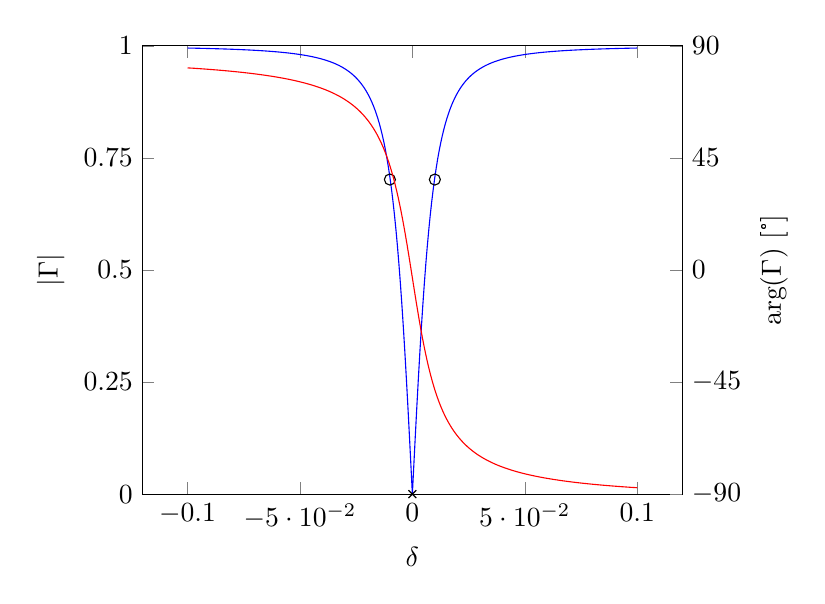
\begin{tikzpicture}[scale=1]
\def\Q0{100}
\begin{axis}[
	  ymin=0,
	  ymax=1,
	  ytick distance=0.25,
	  ylabel={$\vert \Gamma\vert$},
	  xlabel={$\delta$}]
\addplot[mark=x] coordinates {(0,0)};
\addplot[mark=o] coordinates {(1/\Q0,0.7017)};
\addplot[mark=o] coordinates {(-1/\Q0,0.7017)};
\addplot[	blue,
			domain=-10/\Q0:10/\Q0,
		 	mark=none,
		 	samples=301,]{sqrt((\Q0 *x)^2)/(sqrt(1+(\Q0 *x)^2)))};
\end{axis}
\begin{axis}[
	  ymin=-90,
	  ymax=90,
	  ytick distance=45,
      hide x axis,
      axis y line*=right,
      ylabel={$\textrm{arg}(\Gamma)$ [°]},
      ylabel near ticks
    ]
\addplot+[	red,
			domain=-10/\Q0:10/\Q0,
		 	mark=none,
		 	samples=300,]{-3.14-asin(\Q0 *x/sqrt(1+(\Q0 *x)^2))};
		 
		 
\end{axis}
\end{tikzpicture}
\caption{Reflection coefficient of a critically coupled resonator plotted over the detuning factor $\delta$. }\label{fig:resonance}
\end{figure}

\section{Transmission-Type Measurements}

\begin{figure}
\centering
\begin{circuitikz}
\ctikzset {bipoles/length=0.9cm}
%\draw[step=1.0,green,thin] (0,0) grid (10,3);
% Source block
\draw (2,2) to[R=$Y_{01}$,-] (0,2)
			to[sV,v_=$U_s$] (0,0)
			to[short,-] (2,0);
% Transformer 1
\node [] (T1) at (2.75,2) {};
\draw ($(T1)+(-0.75,0)$) to ($(T1)+(-0.3,0)$)
					  to[L,l_=$n_1$] ($(T1)+(-0.3,-2)$)
					  to ($(T1)+(-0.75,-2)$);
\draw ($(T1)+(1.75,0)$) to ($(T1)+(0.3,0)$)
					  to[L,l=$1$,mirror] ($(T1)+(0.3,-2)$)
					  to ($(T1)+(1.75,-2)$);
% RLC circuit
\node [] (RLC) at (5.25,2) {};
\draw ($(RLC)+(-1,0)$) to[short] ($(RLC)+(1,0)$);
\draw ($(RLC)+(-1,-2)$) to[short] ($(RLC)+(1,-2)$);
\draw ($(RLC)+(-1,0)$) to[R=$G$,*-*] ($(RLC)+(-1,-2)$);
\draw (RLC) to[C=$C$,*-*] ($(RLC)+(0,-2)$);
\draw ($(RLC)+(1,0)$) to[L=$L$,*-*] ($(RLC)+(1,-2)$);
\draw ($(RLC)+(0,-2.5)$) node{$Y_R(\delta)$};
% Transformer 2
\node [] (T1) at (8,2) {};
\draw ($(T1)+(-1.75,0)$) to ($(T1)+(-0.3,0)$)
					  to[L,l_=$1$] ($(T1)+(-0.3,-2)$)
					  to ($(T1)+(-1.75,-2)$);
\draw ($(T1)+(0.75,0)$) to ($(T1)+(0.3,0)$)
					  to[L,l=$n_2$,mirror] ($(T1)+(0.3,-2)$)
					  to ($(T1)+(0.75,-2)$);
% Load impedance
\draw (8.75,2) to (9.75,2)
			 to[R=$Y_{02}$] (9.75,0)
			 to (8.75,0);
% Reference planes
\draw [thin,dashed](1.75,-0.5) node[below] {1} -- (1.75,2.5);
\draw [thin,dashed](9,-0.5) node[below] {2} -- (9,2.5);	
		
\end{circuitikz}
\caption{Example for a resonator with two coupling networks.}\label{fig:tr_method}
\end{figure}

As we discussed previously the second method of quality factor measurement methods uses the transmission coefficient to measure the resonances of a cavity. In Fig. \ref{fig:tr_method} an example for a transmission-type measurement is shown, in this example the transmission coefficient $S_{21}$ is measured between reference plane 1 and reference plane 2. This time the resonator is coupled to two ports through two ideal transformers, which as we will find out later are convenient models for coupling loops. These two coupling networks now both load the resonator, so the additional loss introduced by the coupling networks now stems from both ports. The same thing happens to the reactive loading, which now detunes the resonator from both ports. When we take a look at Fig. \ref{fig:norton_tr} we can see that the shunt admittances are transformed into the resonator, where
\begin{align}
Y_1=n_1^2Y_{01}=G_1+jB_1 && Y_2=n_2^2Y_{02}=G_2+jB_2
\end{align}
are the results of this transformation. 

\begin{figure}
\centering
\begin{circuitikz}
\ctikzset {bipoles/length=0.9cm}
%\draw[step=1.0,green,thin] (0,0) grid (10,3);
% Source block
\draw (3.5,0) to[short] (0,0)
		to[american current source=$i_s$] (0,2)
		to[short] (3.5,2);
\draw (1,2) to[R=$G_1$,*-*] (1,0);
\draw (2,2) to[fullgeneric=$jB_1$,*-*] (2,0);
		

% RLC circuit
\node [] (RLC) at (4.5,2) {};
\draw ($(RLC)+(-1,0)$) to[short] ($(RLC)+(1,0)$);
\draw ($(RLC)+(-1,-2)$) to[short] ($(RLC)+(1,-2)$);
\draw ($(RLC)+(-1,0)$) to[R=$G$,*-*] ($(RLC)+(-1,-2)$);
\draw (RLC) to[C=$C$,*-*] ($(RLC)+(0,-2)$);
\draw ($(RLC)+(1,0)$) to[L=$L$,*-*] ($(RLC)+(1,-2)$);
\draw ($(RLC)+(0,-2.5)$) node{$Y_R(\delta)$};
% Load impedance
\draw (5.5,2) to (8,2)
			 to[fullgeneric=$jB_2$] (8,0)
			 to (5.5,0);
\draw (7,2) to[R=$G_2$,*-*] (7,0);		 
			 
		
\end{circuitikz}
\caption{Norton equivalent circuit of Fig. \ref{fig:tr_method}.}\label{fig:norton_tr}
\end{figure}

Like in Fig. \ref{fig:RLC_thevenin} we can use the resonance condition $\Im(Y)=0$ to calculate the loaded resonant frequency $f_L$, where $\delta_L$ is the detuning factor at the loaded resonant frequency. For the loaded quality factor in Equation \eqref{eq:tr_Q_L} we can use the definition for the quality factor to do the same, where a light reactive loading assumption allows us to introduce coupling factors $\kappa_1$ and $\kappa_2$ for port 1 and port 2. 
\begin{equation}
B_1+B_2+G_0Q_0\delta_L=0 \Rightarrow \delta_L(f_L)=-\frac{B_1+B_2}{G_0Q_0}
\end{equation}
\begin{equation}\label{eq:tr_Q_L}
Q_L=\frac{\omega_LC}{G+G_1+G_2}\approx\frac{\omega_0C}{G+G_1+G_2}=Q_0\frac{1}{1+\frac{G_1}{G}+\frac{G_2}{G}}=Q_0\frac{1}{1+\kappa_1+\kappa_2}
\end{equation}

For the transmission coefficient the situation is again very similar. To simplify the matters here we assume that the load and source admittance are both real, i.e. conductances. A meaningful assumption, since the load and source impedances in most of our measurements are more or less conductances as well.
\begin{equation}\label{eq:tr_S}
S_{21}=\frac{2\sqrt{n_1^2Y_{01}n_2^2Y_{02}}}{n_1^2Y_{01}+n_2^2Y_{02}+G(1+jQ_0\delta)}=\frac{2\sqrt{n_1^2Y_{01}n_2^2Y_{02}}}{(n_1^2Y_{01}+n_2^2Y_{02}+G)(1+jQ_L\delta)}
\end{equation}

\begin{equation}
\kappa_1=\frac{n_1^2Y_{01}}{G} \qquad \kappa_2=\frac{n_2^2Y_{02}}{G}
\end{equation}
Having a $(1+jQ\delta)$ factor in the denominator as well, Equation \eqref{eq:tr_S} proves that the transmission coefficient also draws a circle in the complex plane. Like for the reflection coefficient this behaviour is not limited to real reference admittances, but as we will prove in Appendix \ref{app:B} this applies also to the transmission coefficient of any resonator \cite{ginzton}.
\section{Resonance Curve Measurements}\label{sec:rescurve}

\begin{figure}
\centering
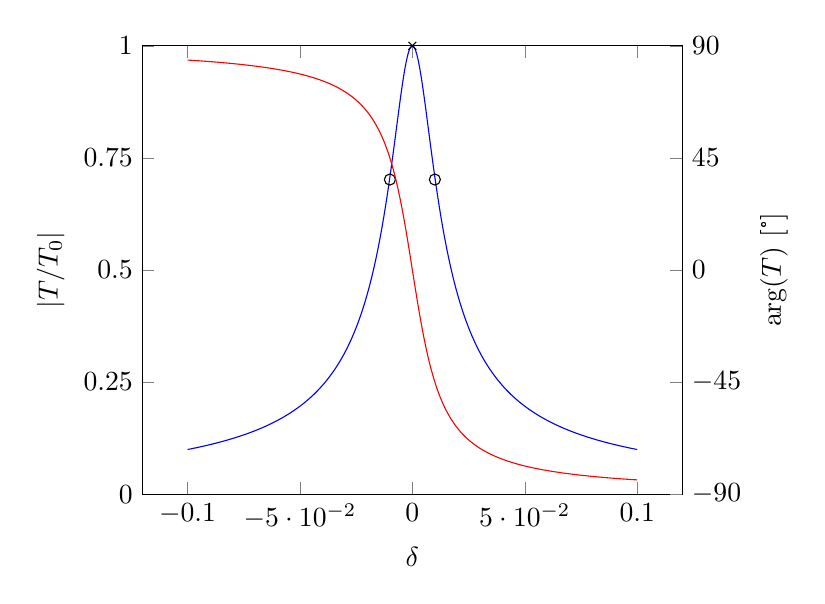
\begin{tikzpicture}[scale=1]
\def\Q0{100}
\begin{axis}[
	  ymin=0,
	  ymax=1,
	  ytick distance=0.25,
	  ylabel={$\vert T/T_0\vert$},
	  xlabel={$\delta$}]
\addplot[mark=x] coordinates {(0,1)};
\addplot[mark=o] coordinates {(1/\Q0,0.7017)};
\addplot[mark=o] coordinates {(-1/\Q0,0.7017)};
\addplot[	blue,
			domain=-10/\Q0:10/\Q0,
		 	mark=none,
		 	samples=301,]{1/(sqrt(1+(\Q0 *x)^2)))};
\end{axis}
\begin{axis}[
	  ymin=-90,
	  ymax=90,
	  ytick distance=45,
      hide x axis,
      axis y line*=right,
      ylabel={$\textrm{arg}(T)$ [°]},
      ylabel near ticks
    ]
\addplot+[	red,
			domain=-10/\Q0:10/\Q0,
		 	mark=none,
		 	samples=300,]{-asin(\Q0 *x/sqrt(1+(\Q0 *x)^2))};
		 
		 
\end{axis}
\end{tikzpicture}
\caption{Typical resonance curve - Transmission coefficient of a undercoupled resonator plotted over the detuning factor $\delta$. }\label{fig:tr_resonance}
\end{figure}

We have now discussed the two fundamental types of resonance measurements. As we have seen, the reflection coefficient and transmission coefficient of both measurement configurations are very similar. Both draw circles in the complex plane due to the $(1+jQ_0\delta)$ factor in their frequency response. This bell-shaped frequency response is characteristic for any resonance in linear circuits. Due to this, the frequency response over the magnitude and the phase is typically used to measure the resonances in a system. Different techniques are used to estimate the quality factor $Q$ and the resonant frequency $\omega_r$ from measured frequency responses, which in turn can be used to calculate the unloaded quality factor $Q_0$ and the unloaded resonant frequency $\omega_0$ if the coupling coefficients of the resonator are known. Most of the algorithms used to estimate the properties of a resonator are fitting techniques that fit the measurements to a known objective function. The parameters of such fits are typically the properties of the resonator or are used to calculate the properties.

The most well-known of these methods is the \textbf{\SI{3}{\decibel} method}. A simple method, which estimates the resonant frequency from the maximum of the magnitude and the quality factor from the \SI{3}{\decibel} bandwidth of the curve. It assumes an undisturbed resonance curve 
\begin{equation}
g(\omega)=\frac{g_0}{\sqrt{1+Q^2(\frac{\omega}{\omega_0}-\frac{\omega_0}{\omega})^2}}\text{,}
\end{equation}
which naturally has its peak magnitude for $g(\omega=\omega_0)=g_0$ at the resonant frequency $\omega_0$. For frequencies $\omega$ close to the resonant frequency $\omega\approx\omega_0$, we can simplify this expression by replacing $\delta$ with its Taylor series around $\omega_0$, $\delta=\omega/\omega_0-\omega_0/\omega\approx 2(\omega/\omega_0-1)$. If we calculate the half-power points of the \SI{3}{\decibel} bandwidth of this simplified expression, we find the quality factor as follows,
\begin{equation}\label{eq:3dB}
\frac{g_0}{\sqrt{2}}=\frac{g_0}{\sqrt{1+4Q^2(\frac{\omega_{3dB}}{\omega_0}-1)^2}} \qquad\Rightarrow\qquad Q=\frac{\omega_0}{2|\omega-\omega_{3dB}|}=\frac{f_0}{2\Delta f}\text{.}
\end{equation}
Obviously, we can approximate the quality factor around the resonant frequency with the ratio resonant frequency $f_0$ over \SI{3}{\decibel} bandwidth $2\Delta f$. This is a very useful results and it can be used to estimate the resonant frequency and the quality factor of a resonance curve. Unfortunately, it is not the most accurate method, since only two or three points of the curve are actually used in the measurement. Today, when we measure resonance curves using a network analyser we measure many more points, so a lot of the available information is not used in the measurement. If the data is noisy, the results of the measurement will be very inaccurate.

Overdetermined measurement methods use many more points and are therefore usually more accurate. These methods are typically computer-based and use linear least-squares or non-linear least-squares fitting algorithms. As the frequency response is a complex function, the magnitude and the phase of the function can be fitted. Algorithms that also fit the phase are circle-fits. All algorithms use the same complex objective function
\begin{equation}
g(\omega)=\frac{g_0}{1+jQ(\frac{\omega}{\omega_0}-\frac{\omega_0}{\omega})}\text{,}
\end{equation}
which must be adapted to each measurement setup. The adaptations compensate for the offset due to coupling, the phase shift on the transmission line, noise and other parasitic influences. Often this is achieved through adding up a suitable polynomial to the objective function.

Petersan and Anlage \cite{petersan} compared the accuracy and precision of seven different methods of determining the resonant frequency and the quality factor, and used both complex data and magnitude data for their comparison. The performance of the methods was compared for different signal-to-noise ratio (SNR) and quality factor values. They found that the most precise methods use complex data and weighting fits, where the latter is used to give noisy data less weight in a fit. In their comparison the phase vs. frequency method - a circle-fit variant - was the most accurate and most precise method for higher SNR values. At the same time a magnitude fit - the Lorentzian fit \cite{bevington} - was the most robust method and provided good results even for very low SNR values. The Lorentzian fit used a Cauchy-Lorentz probability distribution function as approximation to the resonance curve, which was calculated using the same Taylor series for the detuning factor $\delta$ as in the derivation of the 3dB method. Their results (Table \ref{tb:petersan}) also indicated that both methods outperformed the 3dB method in terms of accuracy.

\begin{table}[!htbp]
\centering
{\footnotesize
\begin{tabular}{|c|c|c|c|c|c|c|}
\hline \rule{0pt}{2.6ex}
Method & \multicolumn{2}{c|}{$Q=10^3$} & \multicolumn{2}{c|}{$Q=10^5$} & \multicolumn{2}{c|}{Power ramp ($\text{SNR}\approx 1...2000$)} \\ 
\hline \rule{0pt}{2.6ex}
Type & $Q$ & $f_0$ & $Q$ & $f_0$ & $Q$ & $f_0$ \\ 
\hline \rule{0pt}{2.6ex}
3dB 		& \num{3.29e-2} & \num{1.71e-5} & \num{3.36e-2} & \num{1.71e-7} & \num{12.49} & \num{6.41e-8} \\ 
\hline \rule{0pt}{2.6ex}
Lorentzian 	& \num{2.00e-3} & \num{2.18e-6} & \num{2.09e-3} & \num{2.52e-8} & \textbf{\num{3.11e-2}} & \textbf{\num{1.46e-9}} \\ 
\hline \rule{0pt}{2.6ex}
Phase vs. freq. & \textbf{\num{1.3e-4}} & \textbf{\num{7.88e-8}} & \textbf{\num{1.4e-4}} & \textbf{\num{1.46e-9}} & \num{1.25e-1} & \num{1.75e-8} \\ 
\hline 
\end{tabular}}
\caption{Relative accuracy of 3dB method, Lorentzian method and Phase vs. Freq. method for two values of quality factors ($\text{SNR}=65$), and over different SNR values ($Q=\num{8.71e6}$). Best value in each column is written in bold. Adapted from Petersan and Anlage \cite{petersan}.}\label{tb:petersan}
\end{table}

Although Petersan and Anlage gave a very good overview over the different methods used in measurements, we would like to mention two more methods that were previously used for the split-cylinder resonator. The first method is the \textbf{Coakley method} developed by researchers at the NIST \cite{coakley}. The method, which has strong similarities to the Lorentzian fit, was also used for the measurements in Dr. Janezic's PhD thesis \cite{janezic}. It is a weighted non-linear least-squares technique that uses only the magnitude of the frequency response. Since the convergence of NLLS fits is better for good initial values, the method first approximates the resonant frequency and quality factor using a LS squares method (Estin's method \cite{estin}). Then an initial NLLS fit is made using the objective function 
\begin{equation}
T(f)=\frac{T(f_0)}{1+Q^2(\frac{f}{f_0}-\frac{f_0}{f})^2}+BG\text{.}
\end{equation}
Next the residuals of this fit are squared and put in different equidistant frequency bins. These binned residuals are then used as weights in the final weighted non-linear least squares fit, which yields the resonant frequency and quality factor of the measurement. Being a robust method like the Lorentzian fit, the Coakley method was definitely developed with noisy data of undercoupled resonators in mind.

The second method we would like to mention is the \textbf{Bartley-Begley circle-fit} \cite{bartley}, a modified version of the phase vs. frequency method that is used for the quality factor measurements in the Keysight split-cylinder software. The objective function was merely adjusted to make it suitable for undercoupled resonators,
\begin{equation}
T(f)=L+\frac{de^{-2j\phi}}{1+jQ\left( 2\frac{f-f_0}{f_0}\right) }\text{.}
\end{equation}
The function was linearised, and a complex leakage term and a phase rotation term were added.
\section{Coupling and Measurement Resonators}
While resonators are employed in different kinds of applications like filters or oscillators, the purpose of resonators in complex permittivity measurements is different from these applications. As we only need the properties of the unloaded resonator, we are not interested in transferring high power through the resonator. In the last paragraphs we learned that the amount of power coupled in and out of the resonator depends on the coupling coefficient. Depending on the coupling coefficient, we know three types of coupling:

\begin{center}
\begin{tabular}{c c}
 Under-coupled & $\kappa<1$ \\ 
 Critically-coupled & $\kappa=1$ \\ 
 Over-coupled & $\kappa>1$ \\
\end{tabular}
\end{center}

High-power applications like filters and oscillators are mostly critically coupled or over-coupled, since they want to dissipate more power in the circuitry rather than in the resonator. Of course, one could argue that if we knew the coupling coefficient, measuring with higher power would be better, since we could measure the reflection coefficient or the transmission coefficient with a higher SNR. Unfortunately, measuring the coupling coefficient introduces a great amount of uncertainty as well, since the coupling coefficient is frequency-dependent and is also different for each mode of a cavity. It might be possible to measure $\kappa$ for each mode, but to circumvent the problem altogether we can choose to under-couple the resonator. That means we reduce the coupling for each port so much that $Q_L\approx Q_0$ and $\kappa\approx 0$. This eliminates the influence of the coupling on the quality factor and can - depending on the type of coupling - also reduce the influence on the resonant frequency. Under-coupled resonators are a logical choice for measurement resonators like ours, but the small coupling coefficient can also increase the input impedance of the resonator. This can, as we will see when we discuss the coupling of our resonator, make reflection coefficient measurements very inaccurate, since the accuracy of reflectometers for reflection coefficients close to the unit circle in the Smith chart is very low \cite{pozar,NPL,kajfez}.

\section{Resonance Phenomena and Microwave Cavities}
At the beginning of this chapter we have mentioned that a series or a parallel resonant circuit can be used to model the resonances of a cavity. We have extensively used RLC circuits in this chapter to explain the concepts of quality factor measurements and to show how different measurement methods work. Up to now we have not given any explanation why RLC circuits can be used to model single modes in a cavity. To prove this, we will use a variant of Foster's theorem for distributed circuits, of which waveguides and cavities are prominent examples. Foster's theorem was originally formulated for lumped circuits and states that any lossless, n-mesh circuit with a pair of terminals has an impedance function, which in turn can be represented with n LC circuits in parallel or with n LC circuits in series. An excellent derivation was published by Montogomery et al. \cite{mdp}, which we like to outline here.

If we calculate the input impedance of an arbitrary, lossless one-port with respect to the mean stored magnetic and electric energy in the one-port and the current $i$ flowing through it, we yield Equation \eqref{eq:distr_rlc} for the input impedance.
\begin{equation}\label{eq:distr_rlc}
Z(j\omega)=\frac{j\omega 2(W_H-W_E)}{\frac{1}{2}ii^*}
\end{equation} 
The frequencies for which $W_H=W_E$ are the poles and zeros of Equation \eqref{eq:distr_rlc} and these frequencies are also the resonant frequencies of the one-port. Using Foster's theorem, $Z(j\omega)$ can be expanded into the series
\begin{equation}
Z(j\omega)=j\alpha_1\omega-2\sum\limits_{n=1}^{\infty}r_n\frac{j\omega}{\omega^2-\omega_n^2}\text{,}
\end{equation}
where $\alpha_1$ and $r_n$ are positive constants, and $\omega_n$ are the resonant frequencies of the one-port. As shown in Fig. \ref{fig:foster_ll}, this expansion can be represented by an inductor and an infinite number of LC circuits in series.
\begin{figure}
\centering
\begin{circuitikz}
\ctikzset {bipoles/length=0.9cm}
% First impedances
\draw (0,1) to[L=$L$,o-] +(1.75,0);
% LC circuit
\draw (1.75,1) to[short] +(0.25,0)
			to[short] +(0,0.5)
			to[L=$L_1$] +(1.5,0)
			to[short,-*] +(0,-0.5)
			to[short] +(0.25,0)
			to[short] +(-0.25,0)
			to[short] +(0,-0.5)
			to[C=$C_1$] +(-1.5,0)
			to[short,-*] +(0,0.5);
% LC circuit
\draw (3.75,1) to[short] +(0.25,0)
			to[short] +(0,0.5)
			to[L=$L_2$] +(1.5,0)
			to[short,-*] +(0,-0.5)
			to[short] +(0.25,0)
			to[short] +(-0.25,0)
			to[short] +(0,-0.5)
			to[C=$C_2$] +(-1.5,0)
			to[short,-*] +(0,0.5);
			
\draw[dashed] (5.75,1) -- +(2,0);

% LC circuit
\draw (7.75,1) to[short] +(0.25,0)
			to[short] +(0,0.5)
			to[L=$L$] +(1.5,0)
			to[short,-*] +(0,-0.5)
			to[short] +(0.25,0)
			to[short] +(-0.25,0)
			to[short] +(0,-0.5)
			to[C=$C$] +(-1.5,0)
			to[short,-*] +(0,0.5);
			
\draw (9.75,1) to[short,-o] +(1,0);


\end{circuitikz}
\caption{Foster's equivalent circuit of a lossless one-port, adapted from \cite{mdp}.}\label{fig:foster_ll}
\end{figure}
At frequencies close to the resonant frequency of an LC circuit, i.e close to a pole, the influence of all the other modes diminishes and the value of the impedance is dominated by this LC circuit. Of course, this is only the case, if all other resonant frequencies differ from the resonant frequency compared of the dominant resonance. In an equivalent circuit (Fig. \ref{fig:foster_ll_sr}) the influence of all the other modes is combined to an nearly-constant term $X_k$ and a single LC circuit with resonant frequency $\omega_n$. 

\begin{figure}
\centering
\begin{circuitikz}
\ctikzset {bipoles/length=0.9cm}
% First impedances
\draw (0,1) to[fullgeneric=$X_k$,o-] +(1.75,0);
% LC circuit
\draw (1.75,1) to[short] +(0.25,0)
			to[short] +(0,0.5)
			to[L=$L_1$] +(1.5,0)
			to[short,-*] +(0,-0.5)
			to[short] +(0.25,0)
			to[short] +(-0.25,0)
			to[short] +(0,-0.5)
			to[C=$C_1$] +(-1.5,0)
			to[short,-*] +(0,0.5);
			
\draw (3.75,1) to[short,-o] +(1,0);

\end{circuitikz}
\caption{Equivalent circuit of a single mode, adapted from \cite{mdp}.}\label{fig:foster_ll_sr}
\end{figure}

Until now, we have discussed the situation for lossless circuits, which already illustrates how the impedance of an arbitrary distributed circuit can be described by the poles of the circuit. Although this may be true for lossless circuits, we have ignored that every real circuit is lossy. For slightly lossy circuits Montogomery et al. \cite{mdp} have shown that Foster's theorem applies as well. The derivation for this theorem is similar to the derivation in the lossless case, only this time a complex frequency $\lambda=j\omega+\xi$ is used in the derivation. Interestingly, the theorem breaks down for higher losses, but applies to distributed circuits with low loss. A condition that is conveniently fulfilled by any cavity resonator.
Foster's theorem for slightly lossy distributed circuits shows that any low-loss cavity can be expanded in an infinite number of resonant circuits, where the resonant frequencies of the cavity are the resonant frequencies of the resonant circuits. The equivalent circuit of a cavity developed from the input impedance of a circuit is shown in Fig. \ref{fig:foster_ls} and uses an inductor and lossy parallel resonant circuits for each resonant frequency. A similar development exists for the admittance of a circuit and uses lossy series resonant circuits.
\begin{figure}
\centering
\begin{circuitikz}
\ctikzset {bipoles/length=0.9cm}
% First impedances
\draw (0,1) to[L=$L$,o-] +(1.75,0);
% LC circuit
\draw (1.75,1) to[short] +(0.25,0)
			to[short] +(0,1)
			to[L=$L_1$] +(1.5,0)
			to[short,-*] +(0,-1)
			to[short] +(0.25,0)
			to[short] +(-0.25,0)
			to[short] +(0,-1)
			to[C,l_=$C_1$] +(-1.5,0)
			to[short,-*] +(0,1)
			to[R=$R_1$] +(1.5,0);
% LC circuit
\draw (3.75,1) to[short] +(0.25,0)
			to[short] +(0,1)
			to[L=$L_2$] +(1.5,0)
			to[short,-*] +(0,-1)
			to[short] +(0.25,0)
			to[short] +(-0.25,0)
			to[short] +(0,-1)
			to[C,l_=$C_2$] +(-1.5,0)
			to[short,-*] +(0,1)
			to[R=$R_2$] +(1.5,0);
			
\draw[dashed] (5.75,1) -- +(2,0);

% LC circuit
\draw (7.75,1) to[short] +(0.25,0)
			to[short] +(0,1)
			to[L=$L$] +(1.5,0)
			to[short,-*] +(0,-1)
			to[short] +(0.25,0)
			to[short] +(-0.25,0)
			to[short] +(0,-1)
			to[C,l_=$C$] +(-1.5,0)
			to[short,-*] +(0,1)
			to[R=$R$] +(1.5,0);
			
\draw (9.75,1) to[short,-o] +(1,0);

\end{circuitikz}
\caption{Foster's equivalent circuit of a microwave cavity, adapted from \cite{mdp}.}\label{fig:foster_ls}
\end{figure}
This equivalent circuit (Fig. \ref{fig:foster_ls}) brings us back to the original question we had of how a single resonant circuit could represent a cavity. Again, if we calculate the impedance around a resonant frequency $f_r$ and if all other resonant frequencies are different from this resonant frequency, a single resonance dominates and the contribution for all other modes are so small that they can be modelled by a constant term $X_k$. Clearly, a single mode can be represented by a single resonant circuit and a constant impedance $X_k$, although the constant term is ignored in many instances to simplify the matters even more. (Fig. \ref{fig:foster_ls_sr})
\begin{figure}
\centering
\begin{circuitikz}
\ctikzset {bipoles/length=0.9cm}
% First impedances
\draw (0,1) to[fullgeneric=$X_k$,o-] +(1.75,0);
% LC circuit
\draw (1.75,1) to[short] +(0.25,0)
			to[short] +(0,1)
			to[L=$L$] +(1.5,0)
			to[short,-*] +(0,-1)
			to[short] +(0.25,0)
			to[short] +(-0.25,0)
			to[short] +(0,-1)
			to[C,l_=$C$] +(-1.5,0)
			to[short,-*] +(0,1)
			to[R=$R$] +(1.5,0);
			
\draw (3.75,1) to[short,-o] +(1,0);

\end{circuitikz}
\caption{Equivalent circuit of a single mode of a cavity, adapted from \cite{mdp}.}\label{fig:foster_ls_sr}
\end{figure}

Similar developments exist for multiple terminals as well and we have reasons to believe that resonant circuits are a meaningful way to model the modes in any cavity. The model is still an approximation and it is only valid, if all the other resonant frequencies have different resonant frequencies. If another resonance lies very close to the resonance we want to measure, we would need another resonant circuit for our model to model the interference by another resonance. In many cavities the distances between modes shrink with higher frequencies and there are even cases where so-called degenerate modes have identical resonant frequencies. The split-cylinder resonator is a cylindrical cavity that has certain degenerate $TM$ and $TE$ modes. It is still possible to measure each of these modes, as we have conveniently left out the influence of coupling in these derivations. The terminals we spoke of in connection with Equation \eqref{eq:distr_rlc} were not defined in any way, we can choose them according to our needs, which leads to our next topic, the coupling of cavities.
\section{Coupling of Cavities}\label{sec:cofc}
As we have discussed previously, coupling networks are used to couple energy in and out of a resonant circuit and the degree of coupling is described by the coupling coefficient $\kappa$. In case of a cavity the terminals of the cavity are the terminals of the coupling networks that connect the cavity to the circuit. Each mode has its own coupling coefficient $\kappa_n$, which is defined by how the coupling network interacts with the fields of a mode in the cavity. This interaction is achieved by either inserting parts of the coupling network into the volume of the cavity or by attaching them to the boundaries of the cavity. Unlike in the case of the resonant circuit,  the coupling of a cavity does not only load the resonator, but it also changes the modes inside the resonator. Owing to this mode perturbation, a field calculation must include the coupling networks. Unfortunately, only a few special field problems have simple, analytic solutions, while most problems can only be solved using numerical computations. To avoid these issues coupling networks are often designed as such that they try to disturb the fields inside the cavity as little as possible to approximate the fields with the undisturbed solution. If a coupling network disturbs the fields in a cavity only very little, its coupling coefficient will also be relatively small. A convenient result, since we have already stated that a small coupling coefficient is a good choice for a measurement resonator.
\begin{figure}
  \centering
  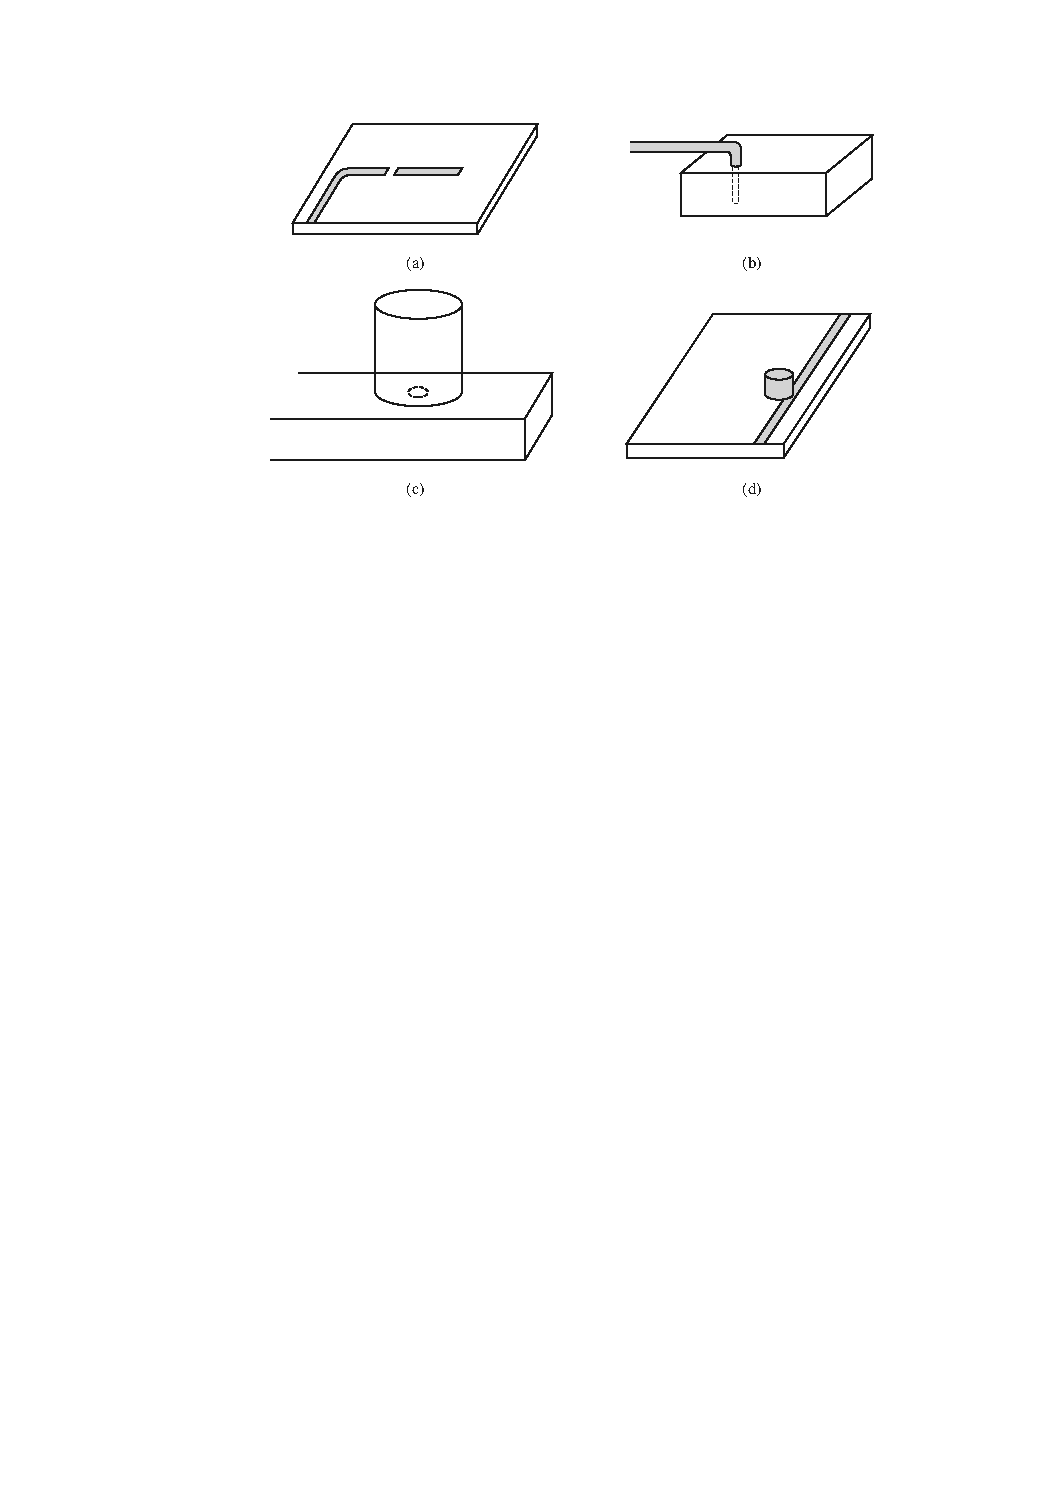
\includegraphics[width=0.7\textwidth]{couplings.pdf}
  \caption{Coupling to microwave resonators, reproduced with permission from \cite{pozar}.}\label{fig:coupling}
\end{figure}

\begin{figure}
\centering
\begin{tikzpicture}
%\draw[step=1cm,gray,very thin] (-3,0) grid (13,7.5);
    \node[anchor=south west,inner sep=0] (image) at (0,0) {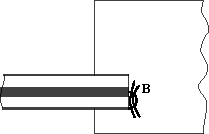
\includegraphics[width=0.4\textwidth]{coupling_loop.pdf}};
    \draw [-latex, thick, red] (1.5,0) node[anchor=east, black] {Coaxial line} to (2.5,0.8);
    \draw [-latex, thick, red] (7,2.5) node[anchor=west, black] {Coupling loop} to (4.25,1);
    \draw [-latex, thick, red] (7,0.4) node[anchor=west, black] {Magnetic field lines} to (4.25,0.75);
    \draw [-latex, thick, red] (2,3) node[anchor=east, black] {Cavity} to (2.9,2.5);
\end{tikzpicture}
\caption{Illustration of a coupling loop.}\label{fig:loop}
\end{figure}

In Fig. \ref{fig:coupling} a few examples for couplings to microwave resonators are shown. Coupling networks usually cater to certain feed lines, modes or desired reactive loads. Fig. \ref{fig:coupling}a shows a gap-coupled microstrip resonator, which couples capacitively from a microstrip to a microstrip resonator. Fig. \ref{fig:coupling}b features an electric probe coupling that couples between a coaxial line and a rectangular waveguide cavity. These two examples were both for (Quasi-)TEM lines, but Fig. \ref{fig:coupling}c exemplifies a rectangular waveguide as feed line and a simple hole in the waveguide as coupling to a cylindrical cavity attached to the waveguide. Finally, Fig. \ref{fig:coupling}d shows a microstrip coupling to a dielectric resonator. Obviously, there is a wide number of different couplings for microwave resonators. For the split-cylinder resonator we have chosen to use magnetic loop coupling (Fig. \ref{fig:loop}). Magnetic loop coupling uses a coaxial line as feed line, which is inserted into the cavity and has the inner conductor connected to either the walls of the cavity or the outer conductor of the feed line. Due to this loop an incident wave creates a loop current in the cavity, which acts more or less like an electrically small magnetic loop antenna.

\begin{figure}
\centering
\begin{circuitikz}
\ctikzset {bipoles/length=0.9cm}
\draw (-2,0) to[short,o-] +(2,0);
% Coupled resonator 1
\draw (0,0) to[short] +(0,-0.25)
			to[L] +(0,-1.5)
			to[short] +(0,-0.25)
			to[open] +(0.5,1.75)
			to[R,l_=$R_1$] +(2,0)
			to[C=$C_1$] +(0,-1.5)
			to[short] +(-2,0)
			to[L,l_=$L_1$] +(0,1.5)
			to[open] +(-0.45,-0.25)
			to [bend left] node[pos=0.5,above] {\tiny $M_{01}$} ++(0.4,0);
% Coupled resonator 2
\draw (0,-2) to[short] +(0,-0.25)
			to[L] +(0,-1.5)
			to[short] +(0,-0.25)
			to[open] +(0.5,1.75)
			to[R,l_=$R_2$] +(2,0)
			to[C=$C_2$] +(0,-1.5)
			to[short] +(-2,0)
			to[L,l_=$L_2$] +(0,1.5)
			to[open] +(-0.45,-0.25)
			to [bend left] node[pos=0.5,above] {\tiny $M_{02}$} ++(0.4,0);
% Dashed line
\draw[dashed] (0,-4) -- +(0,-1);
% Coupled resonator 2
\draw (0,-5) to[short] +(0,-0.25)
			to[L] +(0,-1.5)
			to[short] +(0,-0.25)
			to[open] +(0.5,1.75)
			to[R,l_=$R_n$] +(2,0)
			to[C=$C_n$] +(0,-1.5)
			to[short] +(-2,0)
			to[L,l_=$L_n$] +(0,1.5)
			to[open] +(-0.45,-0.25)
			to [bend left] node[pos=0.5,above] {\tiny $M_{0n}$} ++(0.4,0);
%			
\draw (-2,-7) to[short,o-] +(2,0);

\draw (-1,-3.5) node{$L_0$};



\end{circuitikz}
\caption{Equivalent circuit of a magnetic coupling loop according to \cite{mdp}.}\label{fig:lagrangian}
\end{figure}

Using a Lagrangian method an equivalent circuit (Fig. \ref{fig:lagrangian}) for small loops with an approximately constant loop current can be found \cite{mdp}. The equivalent circuit shows that every mode in the cavity is inductively coupled to the input of the loop by the mutual inductance $M_{0n}$ of a coupled inductor. Equation \eqref{eq:m0n} states that each orthonormal mode $\mathcal{H}_n$ in the cavity with magnetic flux lines running through the loop is coupled out of the cavity. The strength of this coupling depends on the flux running through the loop, the permeability of the field region inside the cavity $\mu$ and the wave number $k_n=\omega_{0n}\sqrt{\epsilon\mu}$.
\begin{equation}\label{eq:m0n}
M_{0n}=\mu k_{0,n}\int\limits_{\mathcal{A}}(\vec{n}\cdot\vec{\mathcal{H}}) dA \qquad \frac{1}{V}\int\limits_{\mathcal{V}}(\vec{\mathcal{H}_n}\cdot\vec{\mathcal{H}_m})dV=\delta_{m,n}
\end{equation}
The other circuit elements of each resonant circuit are defined by the resonant frequency $\omega_{0n}=\frac{1}{\sqrt{L_nC_n}}$ and the quality factor of the mode $Q_n=\frac{\omega_{0n}L_n}{R_n}$, finally the self-inductance of the coupling loop is modelled by the inductor $L_0$.
Regarding the mutual inductance it is interesting to note that the wave number and the permeability are non-zero constants, while the flux through the loop depends on the location and the orientation of coupling loop in the magnetic field. This can be used to amplify or suppress certain modes in a cavity by either locating the coupling loop in an area with a relatively strong field or by turning the loop into the direction of a strong field component. A very useful property, which as we will see in our discussion of the split-cylinder resonator, allows us to separate the transverse magnetic and transverse electric fields of a cavity. 


